\documentclass[tikz]{standalone}
\usepackage{graphicx} % Required for inserting images
\usepackage{tikz}
\usepackage{amsmath}
\usepackage{xcolor}
\usetikzlibrary{ext.paths.ortho} % allows only vertical and horizontal edges
\usetikzlibrary{backgrounds,bending}
\usetikzlibrary{arrows.meta}
\usetikzlibrary {arrows.meta,automata,positioning,fit,calc,matrix,math}
\pgfdeclarelayer{background1}    % Last backgroudn layer
\pgfdeclarelayer{background2}    % Second Last backgroudn layer

\pgfsetlayers{background1,background2,main}  % set the order of the layers (main is the standard layer)

% Custom Color Definition
\definecolor{process_step_background}{HTML}{FFFAF0}
\definecolor{intermediate_fill_colour}{HTML}{949698}
\definecolor{InputOperationColor}{HTML}{99ff99}
\definecolor{OutputOperationColor}{HTML}{FF7F7F}
\tikzset{,line width=5pt}

\tikzstyle{process_step_node} =[fill=process_step_background,rounded corners]
\tikzstyle{OrderOperation} = [fill=white,rounded corners,state,rectangle]
\tikzstyle{InfinitesimalNode}=[circle,draw=none,inner sep=0pt,minimum size=0pt]
\tikzstyle{LabelNode}=[rounded corners,rectangle]


%https://www.ubuntu-user.com/Magazine/Archive/2014/22/Creating-vector-graphics-with-LaTeX-and-TikZ/(offset)/2
\tikzstyle{UpstreamNewProductionEdge}=[rounded corners=10,densely dotted,blue,very thick]
\tikzstyle{UpstreamAdaptionEdge}=[rounded corners=10,loosely dashed,gray,very thick]
\tikzstyle{DownstreamAdaptionEdge}=[rounded corners=10,dashdotdotted,orange,very thick]
\tikzstyle{DownstreamValidationEdge}=[rounded corners=10,brown,very thick]
\tikzstyle{OuterEdges}=[rounded corners=10,very thick]
\begin{document}
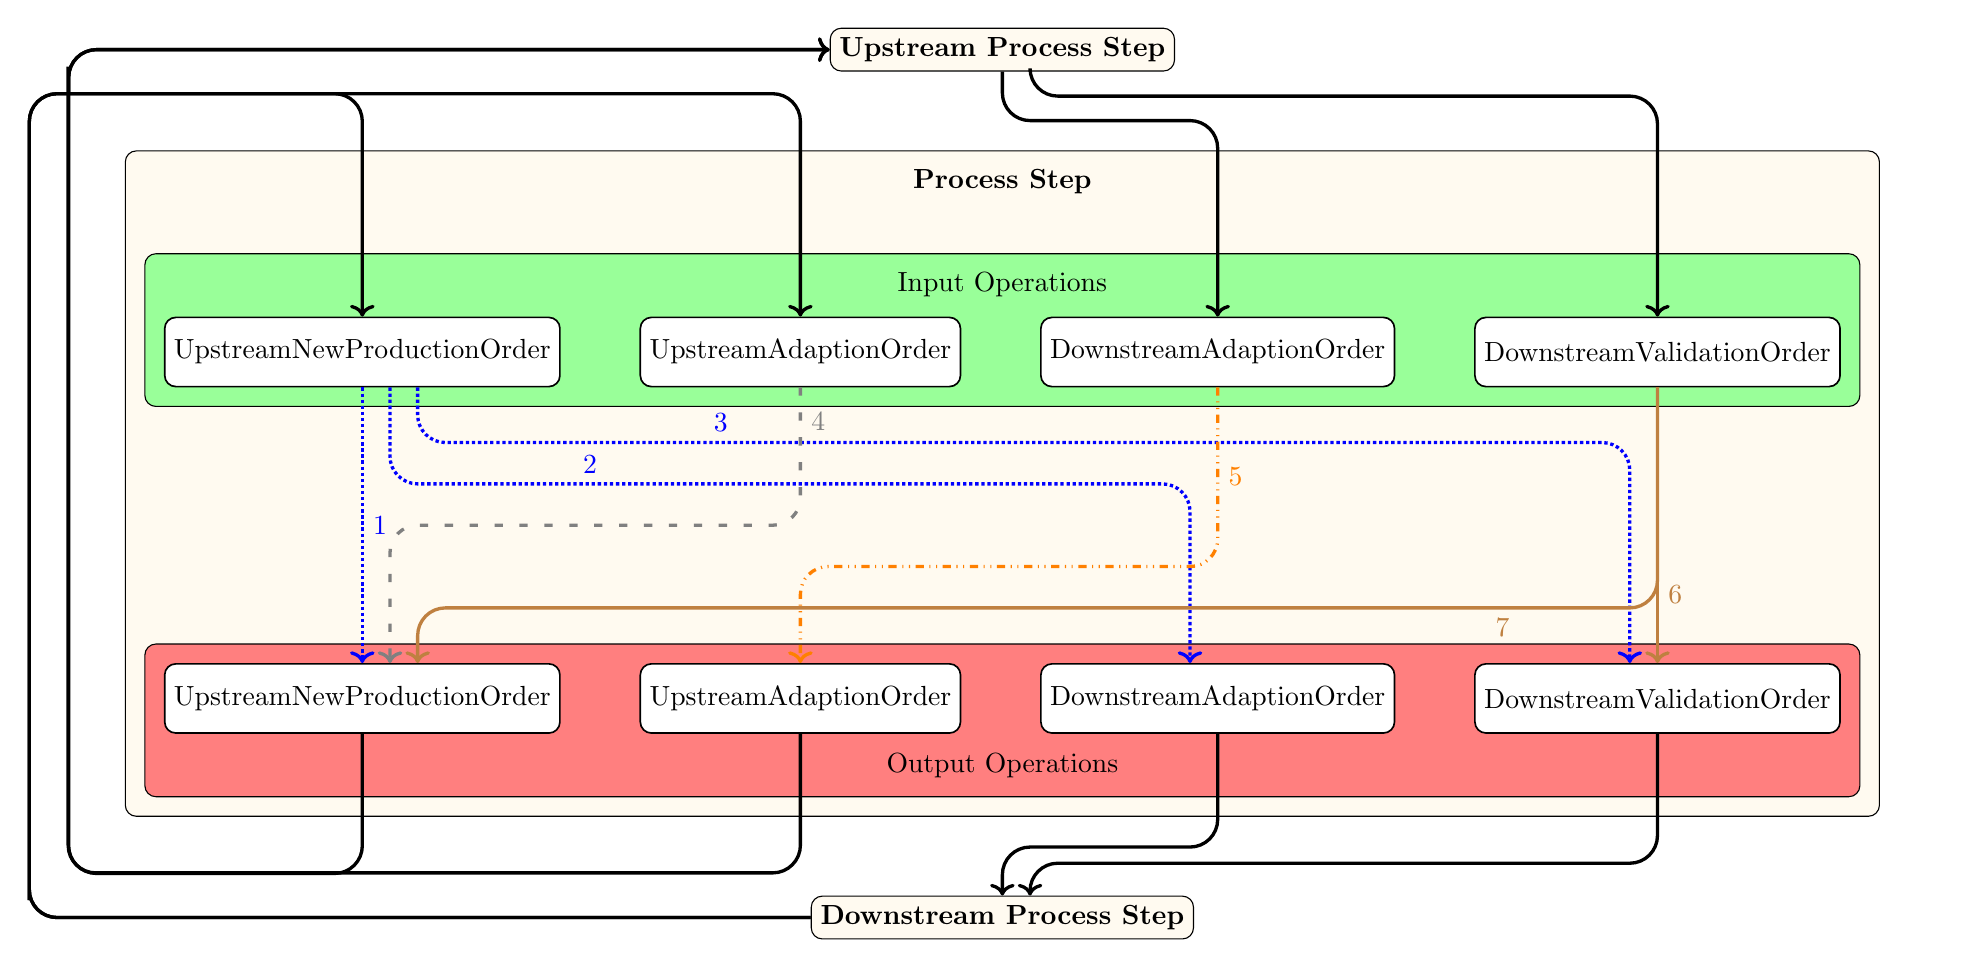
\begin{tikzpicture}[->, auto,node distance=1cm,on grid,semithick]

    %Core Process Step
    %% Inner orders
    \node[OrderOperation](InputUpstreamNewProductionOrder){UpstreamNewProductionOrder};
    \node[OrderOperation,right=of InputUpstreamNewProductionOrder.east](InputUpstreamAdaptionOrder){UpstreamAdaptionOrder};
    \node[OrderOperation,right=of InputUpstreamAdaptionOrder.east](InputDownstreamAdaptionOrder){DownstreamAdaptionOrder};
    \node[OrderOperation,right=of InputDownstreamAdaptionOrder.east](InputDownstreamValidationOrder){DownstreamValidationOrder};

    % \draw (InputDownstreamAdaptionOrder) to coordinate[pos=.5] (OutputDownstreamAdaptionOrder);


    \node[OrderOperation,yshift =-2.5cm,below=of InputUpstreamNewProductionOrder.south](OutputUpstreamNewProductionOrder){UpstreamNewProductionOrder};
    \node[OrderOperation,right=of OutputUpstreamNewProductionOrder.east](OutputUpstreamAdaptionOrder){UpstreamAdaptionOrder};
    \node[OrderOperation,right=of OutputUpstreamAdaptionOrder.east](OutputDownstreamAdaptionOrder){DownstreamAdaptionOrder};
    \node[OrderOperation,right=of OutputDownstreamAdaptionOrder.east](OutputDownstreamValidationOrder){DownstreamValidationOrder};


    %% Inner Input Order Frame
    \begin{pgfonlayer}{background1}
        \node[draw,rounded corners,fit=(InputUpstreamNewProductionOrder)
            (InputUpstreamAdaptionOrder)
            (InputDownstreamAdaptionOrder)
            (InputDownstreamValidationOrder)](InputOrderFrameInvisible){};
    \end{pgfonlayer}
    \node[yshift=-1cm,LabelNode,above= of InputOrderFrameInvisible.north](InputOperationLabelNode){Input Operations};
    \begin{pgfonlayer}{background2}
        \node[draw,fill=InputOperationColor,rounded corners,fit=(InputOrderFrameInvisible)
            (InputOperationLabelNode)
        ](InputOrderFrame){};
    \end{pgfonlayer}

    %% Inner Output Order Frame
    \begin{pgfonlayer}{background1}
        \node[draw,rounded corners,fit=(OutputUpstreamNewProductionOrder)
            (OutputUpstreamAdaptionOrder)
            (OutputDownstreamAdaptionOrder)
            (OutputDownstreamValidationOrder)](OutputOrderFrameInvisible){};
    \end{pgfonlayer}
    \node[yshift=1cm,LabelNode,below= of OutputOrderFrameInvisible.south](OutputOperationLabelNode){Output Operations};

    \begin{pgfonlayer}{background2}
        \node[draw,fill=OutputOperationColor,rounded corners,fit=(OutputOrderFrameInvisible)
            (OutputOperationLabelNode)
        ](OutputOrderFrame){};
    \end{pgfonlayer}

    %% Process Step Frame
    \node[fit=(InputUpstreamNewProductionOrder)
        (InputUpstreamAdaptionOrder)
        (InputDownstreamAdaptionOrder)
        (InputDownstreamValidationOrder)
        (OutputUpstreamNewProductionOrder)
        (OutputUpstreamAdaptionOrder)
        (OutputDownstreamAdaptionOrder)
        (OutputDownstreamValidationOrder)(InputOrderFrame)(OutputOrderFrame)](ProcessStepInvisible){};

    \node[yshift=-0.5 cm,LabelNode,above=of ProcessStepInvisible.north](ProcessStepLabel){\textbf{Process Step}};
    \begin{pgfonlayer}{background1}
        \node[draw,process_step_node,fit=(ProcessStepInvisible)(ProcessStepLabel)](ProcessStepFrame){};
    \end{pgfonlayer}



    %Upstream and DownStream Node
    \node[draw,process_step_node,above=of ProcessStepFrame.north,](UpstreamProcessStep){\textbf{Upstream Process Step}};
    \node[draw,process_step_node,below=of ProcessStepFrame.south](DownstreamProcessStep){\textbf{Downstream Process Step}};


    % Innerpaths
    %% Input UpstreamNewProduction
    \draw[UpstreamNewProductionEdge] (InputUpstreamNewProductionOrder.south) --  (OutputUpstreamNewProductionOrder) node[midway]{1} ;

    \draw[UpstreamNewProductionEdge] ([xshift=20pt]InputUpstreamNewProductionOrder.south) --
    ($([xshift=20pt]InputUpstreamNewProductionOrder.south)!0.2!([xshift=20pt]OutputUpstreamNewProductionOrder.north)$)--
    ($([xshift=-10pt]InputDownstreamValidationOrder.south)!0.2!([xshift=-10pt]OutputDownstreamValidationOrder.north)$) node[near start]{3}--
    ([xshift=-10pt]OutputDownstreamValidationOrder.north) ;
    \draw[UpstreamNewProductionEdge] ([xshift=10pt]InputUpstreamNewProductionOrder.south) --
    ($([xshift=10pt]InputUpstreamNewProductionOrder.south)!0.35!([xshift=10pt]OutputUpstreamNewProductionOrder.north)$) --
    ($([xshift=-10pt]InputDownstreamAdaptionOrder.south)!0.35!([xshift=-10pt]OutputDownstreamAdaptionOrder.north)$) node[near start]{2}--
    ([xshift=-10pt]OutputDownstreamAdaptionOrder.north) ;

    %% InputUpstreamAdaptionOrder 
    \draw[UpstreamAdaptionEdge] (InputUpstreamAdaptionOrder) -- node[near start]{4}
    ($(InputUpstreamAdaptionOrder.south)!0.5!(OutputUpstreamAdaptionOrder.north)$)--
    ($([xshift=10pt]InputUpstreamNewProductionOrder.south)!0.5!([xshift=10pt]OutputUpstreamNewProductionOrder.north)$)--
    ([xshift=10pt]OutputUpstreamNewProductionOrder.north) ;
    %%InputDownstreamAdaptionOrder
    \draw[DownstreamAdaptionEdge] (InputDownstreamAdaptionOrder) -- node[midway]{5}
    ($(InputDownstreamAdaptionOrder.south)!0.65!(OutputDownstreamAdaptionOrder.north)$)--
    ($(InputUpstreamAdaptionOrder.south)!0.65!(OutputUpstreamAdaptionOrder.north)$) --
    (OutputUpstreamAdaptionOrder) ;
    %%InputDownstreamValidationOrder
    \draw[DownstreamValidationEdge] (InputDownstreamValidationOrder) ->  (OutputDownstreamValidationOrder) node[near end]{6};
    \draw[DownstreamValidationEdge] (InputDownstreamValidationOrder.south)--
    ($(InputDownstreamValidationOrder.south)!0.8!(OutputDownstreamValidationOrder.north)$)--
    ($([xshift=20pt]InputUpstreamNewProductionOrder.south)!0.8!([xshift=20pt]OutputUpstreamNewProductionOrder.north)$)node[very near start]{7} --
    ([xshift=20pt]OutputUpstreamNewProductionOrder.north)  ;
    % \path
    % (-2,0) coordinate (v1)
    % (-1,1) coordinate (v2)
    % (0,0)  coordinate (v3)
    % ;
    % %\draw (v1) to[bend left=50] coordinate[pos=.5] (M) (v2);
    % \draw (v1) to coordinate[pos=.5] (M) coordinate[pos=.5] (M);


    %https://tex.stackexchange.com/questions/270604/straight-edge-between-big-nodes-in-tikz
    %Outer Path
    %% Outher Path Nodes

    %%% East nodes
    \node[InfinitesimalNode,below right =of ProcessStepFrame.south east](SouthEastOuterNode){};
    \node[InfinitesimalNode,below right =of ProcessStepFrame.south east,xshift=-0.5cm](SouthEastOuterOuterNode){};
    \node[InfinitesimalNode,above right =of ProcessStepFrame.north east](NorthEastOuterNode){};
    \node[InfinitesimalNode,above right =of ProcessStepFrame.north east,xshift=-0.5cm](NorthEastOuterOuterNode){};

    %%% West nodes
    \node[InfinitesimalNode,below left =of ProcessStepFrame.south west](SouthWestOuterNode){};
    \node[InfinitesimalNode,below left =of ProcessStepFrame.south west,xshift=-0.5cm](SouthWestOuterOuterNode){};
    \node[InfinitesimalNode,above left =of ProcessStepFrame.north west](NorthWestOuterNode){};
    \node[InfinitesimalNode,above left =of ProcessStepFrame.north west,xshift=-0.5cm](NorthWestOuterOuterNode){};








    % East Outer Edges
    \draw[OuterEdges] (OutputDownstreamAdaptionOrder.south) |-|[ratio=.7]  (DownstreamProcessStep.north) node[midway]{};
    \draw[OuterEdges] (OutputDownstreamValidationOrder.south) |-|[ratio=.8]  ([xshift=10pt]DownstreamProcessStep.north) node[midway]{};
    \draw[OuterEdges] (UpstreamProcessStep.south) |-|[ratio=.2]   (InputDownstreamAdaptionOrder.north) node[midway]{};
    \draw[OuterEdges] ([xshift=10pt]UpstreamProcessStep.south) |-|[ratio=.1]  (InputDownstreamValidationOrder.north) node[midway]{};


    % Inv nodes
    \node[InfinitesimalNode,above =of InputUpstreamNewProductionOrder.north,yshift=1.5cm](asdasd){};
    % West Outer Edges

    \draw[OuterEdges] (DownstreamProcessStep.west)-|
    (SouthWestOuterOuterNode.north)-|
    (NorthWestOuterOuterNode.north)-|
    (InputUpstreamNewProductionOrder.north);
    \draw[OuterEdges] (DownstreamProcessStep.west) -|
    (SouthWestOuterOuterNode.north)-|
    (NorthWestOuterOuterNode.north)-|
    (InputUpstreamAdaptionOrder.north);

    \draw[->,OuterEdges] (OutputUpstreamNewProductionOrder.south) |-
    (SouthWestOuterNode.south)|-
    (NorthWestOuterNode.south)|-
    (UpstreamProcessStep.west);
    \draw[->,OuterEdges] (OutputUpstreamAdaptionOrder.south) |-
    (SouthWestOuterNode.west) |-
    (NorthWestOuterNode)|-
    (UpstreamProcessStep.west);



    % \path
    % let \p1 = (SouthEastOuterNode),
    % \p2 =(SouthWestOuterNode),
    % \p3 =(NorthEastOuterNode),
    % \p4=(NorthWestOuterNode),
    % \p5 = (DownstreamProcessStep),
    % \p6 =(UpstreamProcessStep)
    % in
    % coordinate (SouthEastPoint) at (\x1,\y1);

    % \draw let
    % \p1 = (SouthEastOuterNode),
    % \p2 =(SouthWestOuterNode),
    % \p5 = (DownstreamProcessStep.south east),
    % \p6 =(OutputDownstreamAdaptionOrder)
    % in
    % (OutputDownstreamAdaptionOrder)  -- (\x6,\y1)
    % (\x6,\y1) -- (\x5,\y1);


\end{tikzpicture}
\end{document}
